% This LaTeX was auto-generated from MATLAB code.
% To make changes, update the MATLAB code and export to LaTeX again.

\documentclass{article}

\usepackage[utf8]{inputenc}
\usepackage[T1]{fontenc}
\usepackage{lmodern}
\usepackage{graphicx}
\usepackage{color}
\usepackage{hyperref}
\usepackage{amsmath}
\usepackage{amsfonts}
\usepackage{epstopdf}
\usepackage[table]{xcolor}
\usepackage{matlab}

\sloppy
\epstopdfsetup{outdir=./}
\graphicspath{ {./Final_1_images/} }

\begin{document}

\matlabtitle{Manipulation Estimation and Controls: Assignment 1}

\begin{par}
\begin{flushleft}
Submitted by: Sushanth Jayanth
\end{flushleft}
\end{par}

\matlabheading{Q1. }

\begin{par}
\begin{flushleft}
\textbf{Linear system is defined with in the form x = Ax + Bu}
\end{flushleft}
\end{par}

\begin{par}
\begin{flushleft}
Where A and B are defined as
\end{flushleft}
\end{par}

\begin{matlabcode}
A = [[0,1,0];[0,0,1];[1,5,7]];
B = transpose([1,0,0]);
C = [0,1,3];
\end{matlabcode}

\begin{par}
\begin{flushleft}
  
\end{flushleft}
\end{par}

\matlabheadingthree{ 1 a. Stability Criterion for the above system is defined by the eigenvalues of A}

\begin{par}
\hfill \break
\end{par}

\begin{matlabcode}
eigen_A = eig(A)
\end{matlabcode}
\begin{matlaboutput}
eigen_A = 3x1 complex    
   7.6690 + 0.0000i
  -0.3345 + 0.1361i
  -0.3345 - 0.1361i

\end{matlaboutput}

\begin{par}
\begin{flushleft}
    Since one of the eigen values is positive, the linear system A is unstable
\end{flushleft}
\end{par}


\vspace{1em}
\matlabheadingthree{  1  b. Controllability of the system}

\begin{par}
\hfill \break
\end{par}

\begin{matlabcode}
Q = ctrb(A,B)
\end{matlabcode}
\begin{matlaboutput}
Q = 3x3    
     1     0     0
     0     0     1
     0     1     7

\end{matlaboutput}
\begin{matlabcode}
clear rank
rank_of_Q = rank(Q)
\end{matlabcode}
\begin{matlaboutput}
rank_of_Q = 3
\end{matlaboutput}

\begin{par}
\begin{flushleft}
  Matrix Q is of rank n (same rank as of A). Therefore the system is controllable
\end{flushleft}
\end{par}


\vspace{1em}
\matlabheadingthree{ 1  c. Initial State Vector is given as: }

\begin{par}
\begin{flushleft}
 The output of the unforced system plotted below:
\end{flushleft}
\end{par}

\begin{matlabcode}
x_0 = [0;1;0]
\end{matlabcode}
\begin{matlaboutput}
x_0 = 3x1    
     0
     1
     0

\end{matlaboutput}
\begin{matlabcode}

syms t
fplot(C*expm(A*t)*x_0, [0,2])
\end{matlabcode}
\begin{center}
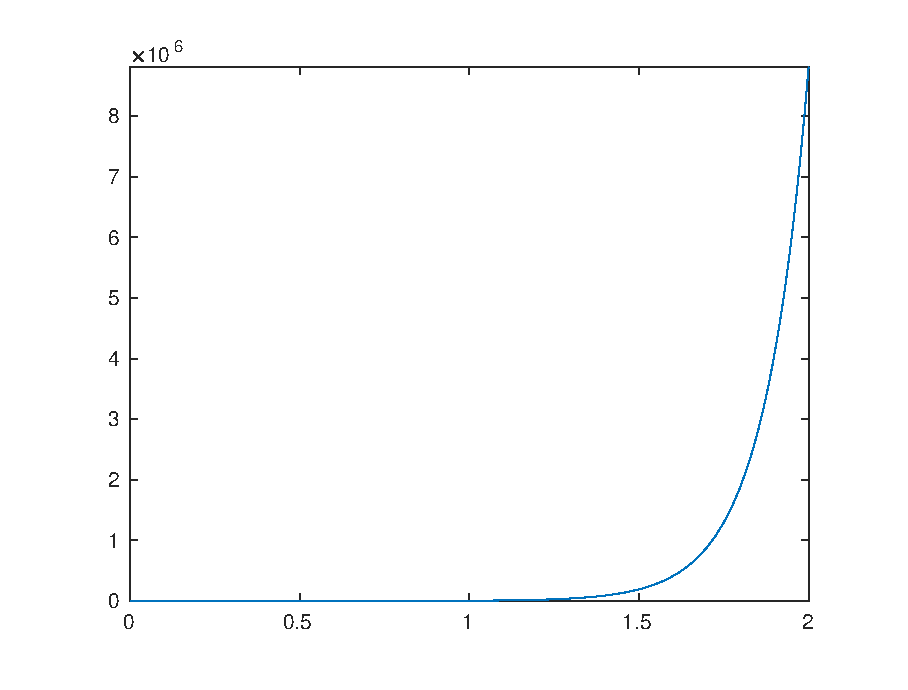
\includegraphics[width=\maxwidth{83.69292523833417em}]{figure_0.eps}
\end{center}


\vspace{1em}
\matlabheadingthree{ 1  d. Find the feedback gain K to make the system stable}

\begin{par}
\hfill \break
\end{par}

\begin{matlabcode}
eig_values = [-1 + 1i, -1 - 1i, -2]
\end{matlabcode}
\begin{matlaboutput}
eig_values = 1x3 complex    
  -1.0000 + 1.0000i  -1.0000 - 1.0000i  -2.0000 + 0.0000i

\end{matlaboutput}
\begin{matlabcode}
K = place(A,B,eig_values)
\end{matlabcode}
\begin{matlaboutput}
K = 1x3    
   11.0000   60.0000   88.0000

\end{matlaboutput}


\vspace{1em}
\matlabheadingthree{   1 e. Plot output of the system after control input}

\begin{par}
\hfill \break
\end{par}

\begin{matlabcode}
new_mat = A-B*K
\end{matlabcode}
\begin{matlaboutput}
new_mat = 3x3    
  -11.0000  -59.0000  -88.0000
         0         0    1.0000
    1.0000    5.0000    7.0000

\end{matlaboutput}
\begin{matlabcode}
fplot(C*expm(new_mat*t)*x_0, [0,10])
\end{matlabcode}
\begin{center}
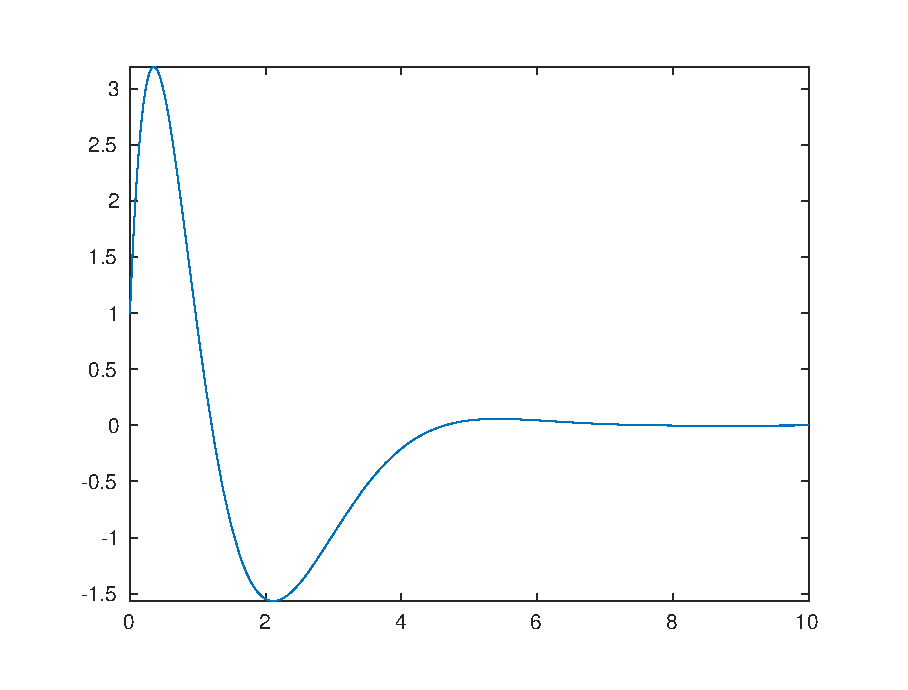
\includegraphics[width=\maxwidth{83.69292523833417em}]{figure_1.eps}
\end{center}


\vspace{1em}

\matlabheading{Q 2. }

\matlabheadingthree{\textbf{"Pendulum on a cart" system}}

\matlabheadingthree{2 a. Cart pendulum equations as non-linear state-space equations}

\begin{par}
\begin{flushleft}
Cart pendulum equations are written as shown below:
\end{flushleft}
\end{par}

\begin{matlabcode}
syms F
syms z
F = gamma*xc_ddot - beta*phi_ddot*cos(phi) + beta*phi_dot*phi_dot*sin(phi) + mu*xc_dot % = F
\end{matlabcode}
\begin{matlabsymbolicoutput}
F = 

\hskip1em $\displaystyle \beta \,\sin \left(\phi \right)\,{\dot{\phi} }^2 +\gamma \,\ddot{\textrm{xc}} +\mu \,\dot{\textrm{xc}} -\beta \,\ddot{\phi} \,\cos \left(\phi \right)$
\end{matlabsymbolicoutput}
\begin{matlabcode}

z = 0
\end{matlabcode}
\begin{matlaboutput}
z = 0
\end{matlaboutput}
\begin{matlabcode}
z = alpha*phi_ddot - beta*xc_ddot*cos(phi) - D*sin(phi)
\end{matlabcode}
\begin{matlabsymbolicoutput}
z = 

\hskip1em $\displaystyle \alpha \,\ddot{\phi} -\textrm{D}\,\sin \left(\phi \right)-\beta \,\ddot{\textrm{xc}} \,\cos \left(\phi \right)$
\end{matlabsymbolicoutput}

\begin{par}
\begin{flushleft}
The state vector x is given as:
\end{flushleft}
\end{par}

\begin{matlabcode}
syms xc_ddot xc_dot xc gamma beta phi phi_dot phi_ddot mu alpha D u 
x = [xc; phi; xc_dot; phi_dot]
\end{matlabcode}
\begin{matlabsymbolicoutput}
x = 

\hskip1em $\displaystyle \left(\begin{array}{c}
\textrm{xc}\\
\phi \\
\dot{\textrm{xc}} \\
\dot{\phi} 
\end{array}\right)$
\end{matlabsymbolicoutput}

\begin{par}
\begin{flushleft}
The standard mechanical form is given as:
\end{flushleft}
\end{par}

\begin{par}
\begin{flushleft}
\includegraphics[width=\maxwidth{30.406422478675363em}]{image_0}
\end{flushleft}
\end{par}

\begin{par}
\begin{flushleft}
The state-space representation of the standard mechanical form is given as:
\end{flushleft}
\end{par}

\begin{par}
\begin{flushleft}
\includegraphics[width=\maxwidth{35.52433517310587em}]{image_1}
\end{flushleft}
\end{par}

\begin{par}
\begin{flushleft}
The derivation of the above equation is shown below:
\end{flushleft}
\end{par}

\begin{matlabcode}
syms xc_ddot xc_dot xc gamma beta phi phi_dot phi_ddot mu alpha D u 

M = [[gamma, -beta*cos(phi)];[-beta*cos(phi),alpha]]
\end{matlabcode}
\begin{matlabsymbolicoutput}
M = 

\hskip1em $\displaystyle \left(\begin{array}{cc}
\gamma  & -\beta \,\cos \left(\phi \right)\\
-\beta \,\cos \left(\phi \right) & \alpha 
\end{array}\right)$
\end{matlabsymbolicoutput}
\begin{matlabcode}
C = [beta*phi_dot*phi_dot*sin(phi) + mu*xc_dot; 0]
\end{matlabcode}
\begin{matlabsymbolicoutput}
C = 

\hskip1em $\displaystyle \left(\begin{array}{c}
\beta \,\sin \left(\phi \right)\,{\dot{\phi} }^2 +\mu \,\dot{\textrm{xc}} \\
0
\end{array}\right)$
\end{matlabsymbolicoutput}
\begin{matlabcode}
G = [0; -D*sin(phi)]
\end{matlabcode}
\begin{matlabsymbolicoutput}
G = 

\hskip1em $\displaystyle \left(\begin{array}{c}
0\\
-\textrm{D}\,\sin \left(\phi \right)
\end{array}\right)$
\end{matlabsymbolicoutput}
\begin{matlabcode}
U = [u; 0]
\end{matlabcode}
\begin{matlabsymbolicoutput}
U = 

\hskip1em $\displaystyle \left(\begin{array}{c}
u\\
0
\end{array}\right)$
\end{matlabsymbolicoutput}
\begin{matlabcode}

q_dd = inv(M)*(u - G - C)
\end{matlabcode}
\begin{matlabsymbolicoutput}
q\_dd = 

\hskip1em $\displaystyle \begin{array}{l}
\left(\begin{array}{c}
\frac{\beta \,\cos \left(\phi \right)\,{\left(u+\textrm{D}\,\sin \left(\phi \right)\right)}}{\sigma_1 }-\frac{\alpha \,{\left(\beta \,\sin \left(\phi \right)\,{\dot{\phi} }^2 -u+\mu \,\dot{\textrm{xc}} \right)}}{\sigma_1 }\\
\frac{\gamma \,{\left(u+\textrm{D}\,\sin \left(\phi \right)\right)}}{\sigma_1 }-\frac{\beta \,\cos \left(\phi \right)\,{\left(\beta \,\sin \left(\phi \right)\,{\dot{\phi} }^2 -u+\mu \,\dot{\textrm{xc}} \right)}}{\sigma_1 }
\end{array}\right)\\
\mathrm{}\\
\textrm{where}\\
\mathrm{}\\
\;\;\sigma_1 =\alpha \,\gamma -\beta^2 \,{\cos \left(\phi \right)}^2 
\end{array}$
\end{matlabsymbolicoutput}
\begin{matlabcode}

state_space_form = [xc_dot; phi_dot; q_dd]
\end{matlabcode}
\begin{matlabsymbolicoutput}
state\_space\_form = 

\hskip1em $\displaystyle \begin{array}{l}
\left(\begin{array}{c}
\dot{\textrm{xc}} \\
\dot{\phi} \\
\frac{\beta \,\cos \left(\phi \right)\,{\left(u+\textrm{D}\,\sin \left(\phi \right)\right)}}{\sigma_1 }-\frac{\alpha \,{\left(\beta \,\sin \left(\phi \right)\,{\dot{\phi} }^2 -u+\mu \,\dot{\textrm{xc}} \right)}}{\sigma_1 }\\
\frac{\gamma \,{\left(u+\textrm{D}\,\sin \left(\phi \right)\right)}}{\sigma_1 }-\frac{\beta \,\cos \left(\phi \right)\,{\left(\beta \,\sin \left(\phi \right)\,{\dot{\phi} }^2 -u+\mu \,\dot{\textrm{xc}} \right)}}{\sigma_1 }
\end{array}\right)\\
\mathrm{}\\
\textrm{where}\\
\mathrm{}\\
\;\;\sigma_1 =\alpha \,\gamma -\beta^2 \,{\cos \left(\phi \right)}^2 
\end{array}$
\end{matlabsymbolicoutput}


\vspace{1em}
\matlabheadingthree{2 b. Describe the set of equilibrium points}

\begin{par}
\begin{flushleft}
\includegraphics[width=\maxwidth{69.24234821876568em}]{image_2}
\end{flushleft}
\end{par}

\begin{par}
\begin{flushleft}
\includegraphics[width=\maxwidth{69.34269944806825em}]{image_3}
\end{flushleft}
\end{par}

\begin{par}
\begin{flushleft}
\includegraphics[width=\maxwidth{69.34269944806825em}]{image_4}
\end{flushleft}
\end{par}

\vspace{1em}

\matlabheadingthree{2 c. Compute the eigen values of matrix A which represents the linearized system about the equilibrium point at x = 0}

\begin{par}
\hfill \break
\end{par}

\begin{matlabcode}
A = [[0,0,1,0];[0,0,0,1];[0,1,-3,0];[0,2,-3,0]];

B = [0;0;1;1];

eig_A = eig(A)
\end{matlabcode}
\begin{matlaboutput}
eig_A = 4x1    
         0
   -3.3301
    1.1284
   -0.7984

\end{matlaboutput}

\begin{par}
\begin{flushleft}
Since one the eigenvalues of A have a real positive value the system is unstable about the state x = 0
\end{flushleft}
\end{par}

\begin{par}
\begin{flushleft}
This means that the vertical upright pendulum is not in stable equilibrium
\end{flushleft}
\end{par}


\vspace{1em}
\matlabheadingthree{ \textbf{2 d. Finding the optimal feedback control gain }}

\begin{par}
\hfill \break
\end{par}

\begin{matlabcode}
Q = [[1,0,0,0];[0,5,0,0];[0,0,1,0];[0,0,0,5]];
R = 10;

K = lqr(A, B, Q, R)
\end{matlabcode}
\begin{matlaboutput}
K = 1x4    
   -0.3162   10.2723   -6.7857    9.2183

\end{matlaboutput}

\begin{par}
\begin{flushleft}
 Using the above feedback control to plot the state of the linearized system
\end{flushleft}
\end{par}

\begin{matlabcode}
t = 0 : 0.01 : 30 ;

% define three initial state vectors x_0, x_1, and x_2
x_0 = [0; 0.1; 0; 0];
x_1 = [0; 0.5; 0; 0];
x_2 = [0; 1.0886; 0; 0];
x_3 = [0; 1.1; 0; 0];

% plotting the state of system beginning at x_0
[t,x0] = ode45(@(t,x)(A-B*K)*x, t, x_0);
plot(t0,x0)
title('state of system beginning at x_0')
ylabel('Amplitude')
xlabel('time(s)')
\end{matlabcode}
\begin{center}
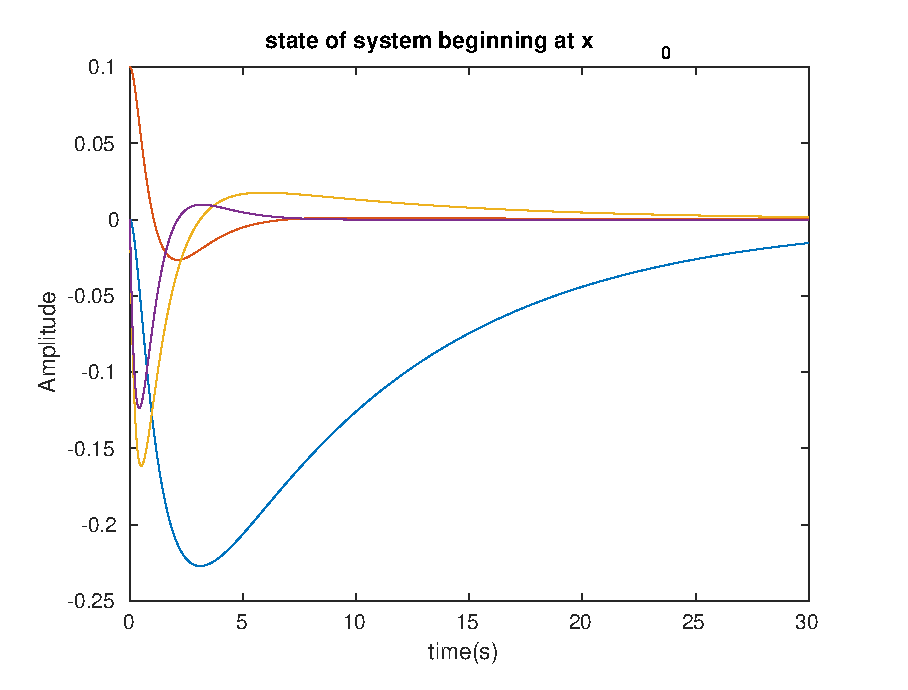
\includegraphics[width=\maxwidth{83.69292523833417em}]{figure_2.eps}
\end{center}
\begin{matlabcode}

% plotting the state of system beginning at x_1
[t,x1] = ode45(@(t,x)(A-B*K)*x, t, x_1);
plot(t,x1)
title('state of system beginning at x_1')
ylabel('Amplitude')
xlabel('time(s)')
\end{matlabcode}
\begin{center}
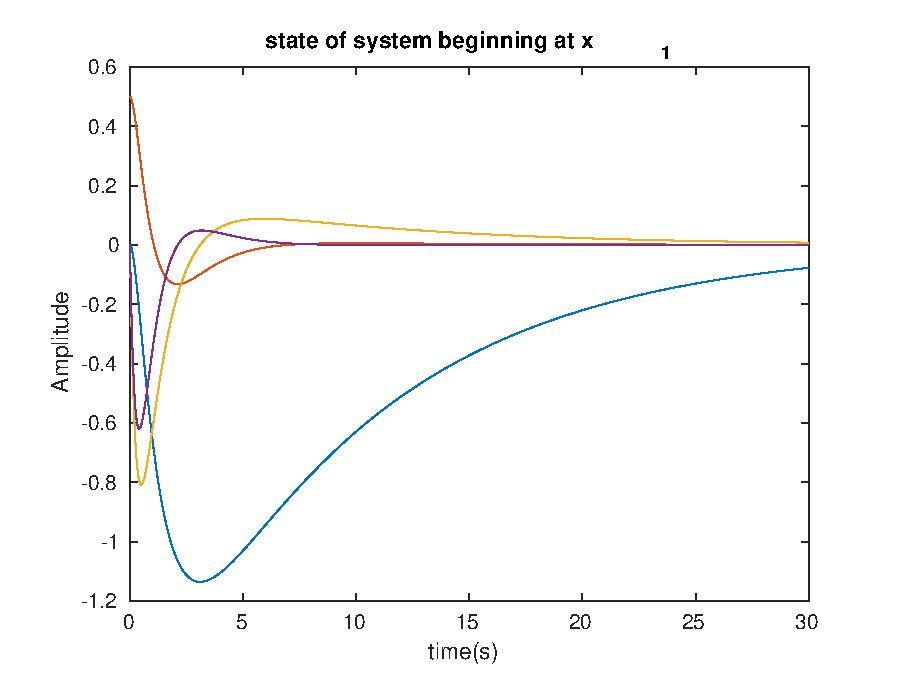
\includegraphics[width=\maxwidth{83.69292523833417em}]{figure_3.eps}
\end{center}
\begin{matlabcode}

% plotting the state of system beginning at x_2
[t,x2] = ode45(@(t,x)(A-B*K)*x, t, x_2);
plot(t,x2)
title('state of system beginning at x_2')
ylabel('Amplitude')
xlabel('time(s)')
\end{matlabcode}
\begin{center}
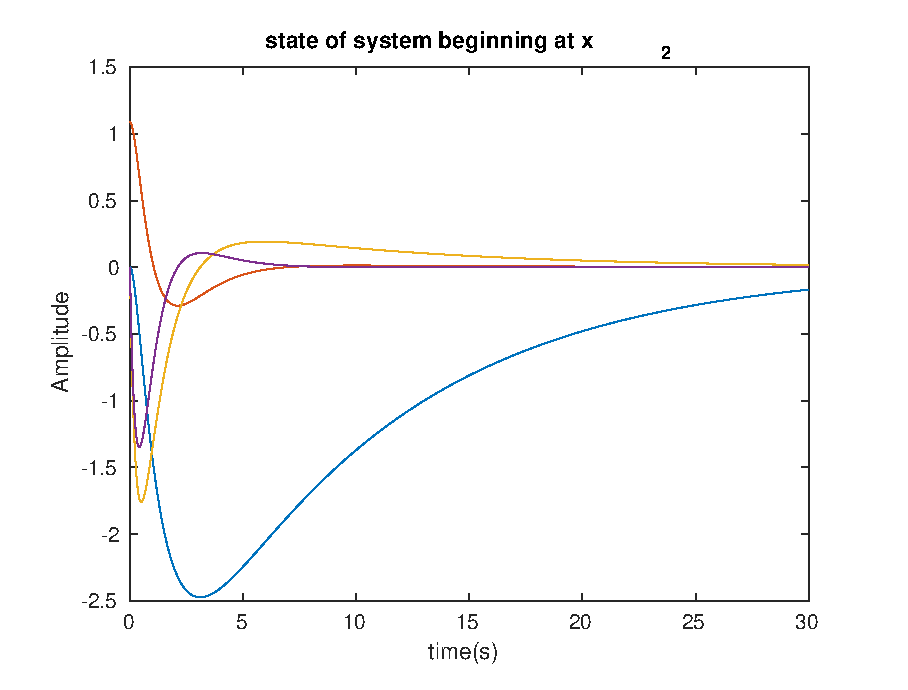
\includegraphics[width=\maxwidth{83.69292523833417em}]{figure_4.eps}
\end{center}
\begin{matlabcode}

% plotting the state of system beginning at x_0
[t,x3] = ode45(@(t,x)(A-B*K)*x, t, x_3);
plot(t,x0)
title('state of system beginning at x_3')
ylabel('Amplitude')
xlabel('time(s)')
\end{matlabcode}
\begin{center}
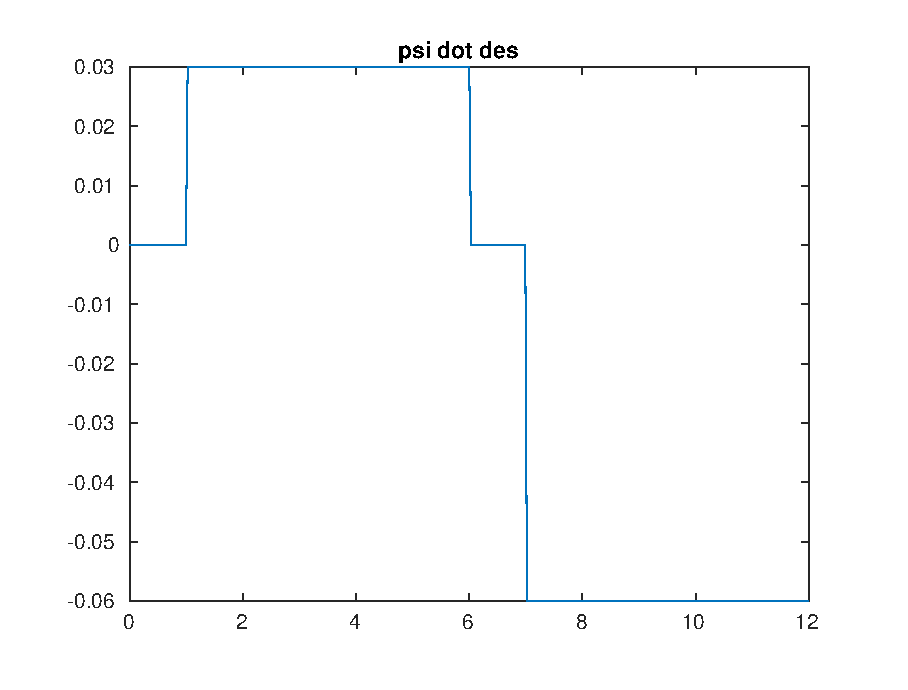
\includegraphics[width=\maxwidth{83.69292523833417em}]{figure_5.eps}
\end{center}


\vspace{1em}
\begin{par}
\begin{flushleft}
\textbf{2 e. Repeat 2 d. using non-linearized state equations}
\end{flushleft}
\end{par}

\begin{par}
\begin{flushleft}
The non linear system is computed below:
\end{flushleft}
\end{par}

\begin{matlabcode}
[t,x4] = ode45(@(t,x4)(non_linear_fun(x4, -K*x4)), t, x_0);
plot(t, x4)
title('state of non-linear system beginning at x_0')
ylabel('Amplitude')
xlabel('time(s)')
\end{matlabcode}
\begin{center}
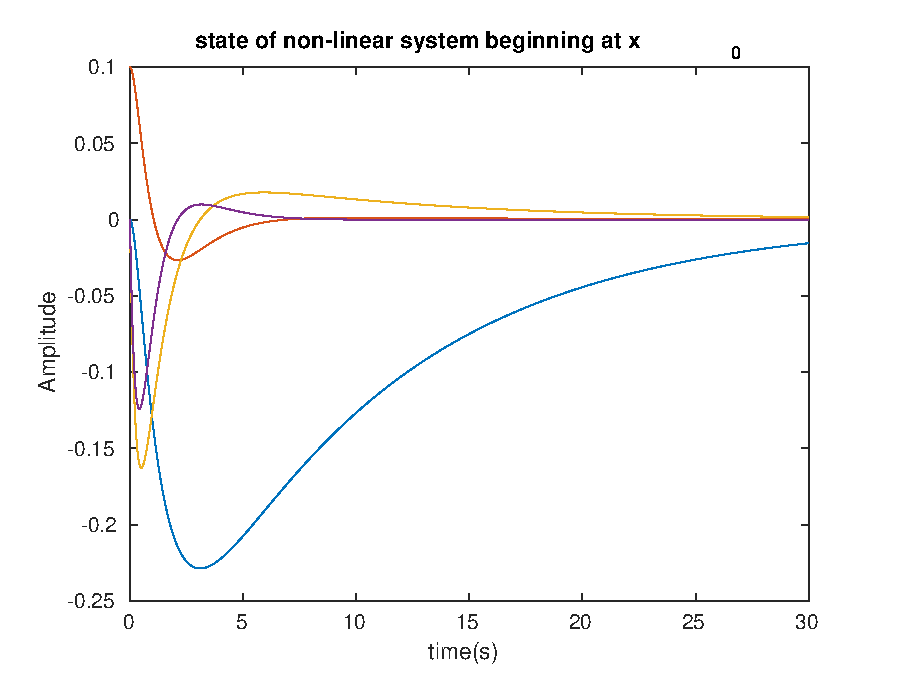
\includegraphics[width=\maxwidth{83.69292523833417em}]{figure_6.eps}
\end{center}
\begin{matlabcode}

[t,x4] = ode45(@(t,x4)(non_linear_fun(x4, -K*x4)), t, x_2);
plot(t, x4)
title('state of non-linear system beginning at x_2')
ylabel('Amplitude')
xlabel('time(s)')
\end{matlabcode}
\begin{center}
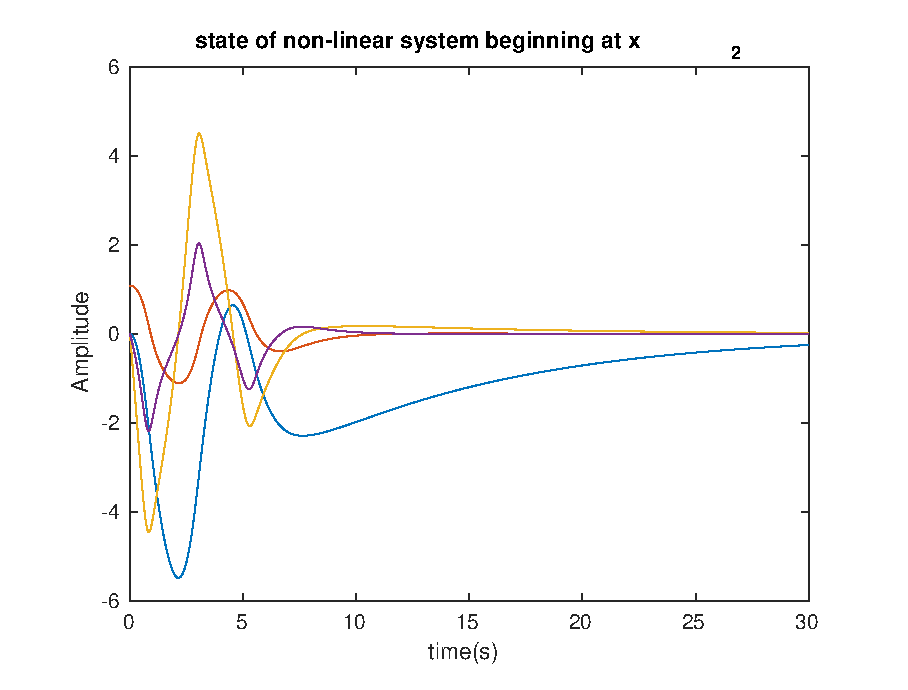
\includegraphics[width=\maxwidth{83.69292523833417em}]{figure_7.eps}
\end{center}
\begin{matlabcode}

[t,x4] = ode45(@(t,x4)(non_linear_fun(x4, -K*x4)), t, x_3);
\end{matlabcode}
\begin{matlaboutput}
Warning: Failure at t=9.394808e+00.  Unable to meet integration tolerances without reducing the step size below the smallest value allowed (2.842171e-14) at time t.
\end{matlaboutput}
\begin{matlabcode}
plot(t, x4)
title('state of non-linear system beginning at x_3')
ylabel('Amplitude')
xlabel('time(s)')
\end{matlabcode}
\begin{center}
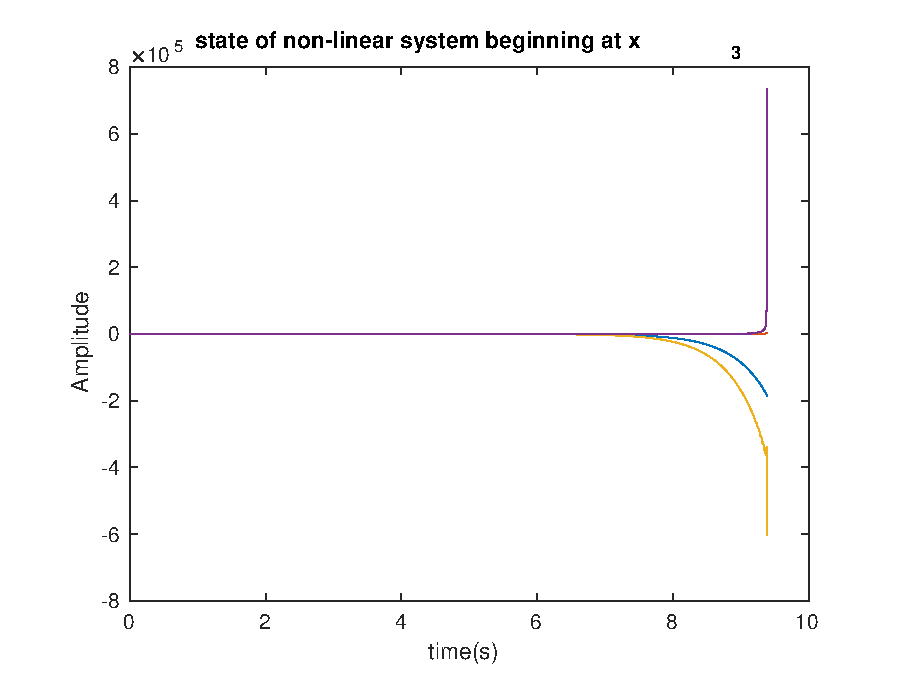
\includegraphics[width=\maxwidth{83.69292523833417em}]{figure_8.eps}
\end{center}

\begin{par}
\begin{flushleft}
The non-linear system is not stable when the initial state vector has a high value of x\_c as in the case of x\_3 = [0; 1.1; 0; 0]
\end{flushleft}
\end{par}


\vspace{1em}
\begin{par}
\begin{flushleft}
\textbf{2 f. Find the matrix C to sensor measurements in y are in inches ( y = Cx )}
\end{flushleft}
\end{par}

\begin{par}
\begin{flushleft}
y measures only position therefore should have a dimension of (1,) i.e is a scalar
\end{flushleft}
\end{par}

\begin{par}
\begin{flushleft}
x = [ x; ϕ; x'; ϕ'] and has shape (4,1)
\end{flushleft}
\end{par}

\begin{par}
\begin{flushleft}
Therefore C must have shape (1,4)
\end{flushleft}
\end{par}

\begin{matlabcode}
% Finding C from above equation

% 1 metre = 39.3701 inches, therefore C must be

C = [39.3701, 0, 0, 0]
\end{matlabcode}
\begin{matlaboutput}
C = 1x4    
   39.3701         0         0         0

\end{matlaboutput}


\vspace{1em}
\begin{par}
\begin{flushleft}
\textbf{2 g. Create a tracking controller to specify a desired cart position trajectory}
\end{flushleft}
\end{par}

\begin{par}
\begin{flushleft}
A tracking controller is represented as:
\end{flushleft}
\end{par}

\begin{par}
\begin{flushleft}
\includegraphics[width=\maxwidth{80.6823883592574em}]{image_5}
\end{flushleft}
\end{par}

\begin{par}
\begin{flushleft}
\includegraphics[width=\maxwidth{35.22328148519819em}]{image_6}
\end{flushleft}
\end{par}

\begin{matlabcode}
% Defining the specified timesteps and duration
t_5 = 0 : 0.01 : 200;
x_5 = [0; 0; 0; 0];
K % from previous LQR caluculation
\end{matlabcode}
\begin{matlaboutput}
K = 1x4    
   -0.3162   10.2723   -6.7857    9.2183

\end{matlaboutput}
\begin{matlabcode}

% define parameters for y_des only for plotting
freq=0.01;
offset=0;
amp=20;
duty=50;

% define y_des as a square wave function
y_des = offset+amp*square(2*pi*freq.*t_5,duty);

v = -1 * inv(C*inv((A-B*K))*B);

[t,x5] = ode45(@(t,x5)(tracking_controller(x5, -K*x5, v, t)), t_5, x_5);
% since y_des is in inches and x5 is in metres, we multiply the x5 plot
plot(t, x5*39.3701)
hold on
plot(t_5,y_des)
hold off
title('tracking controller with given Q,R values')
ylabel('Amplitude')
xlabel('time(s)')
\end{matlabcode}
\begin{center}
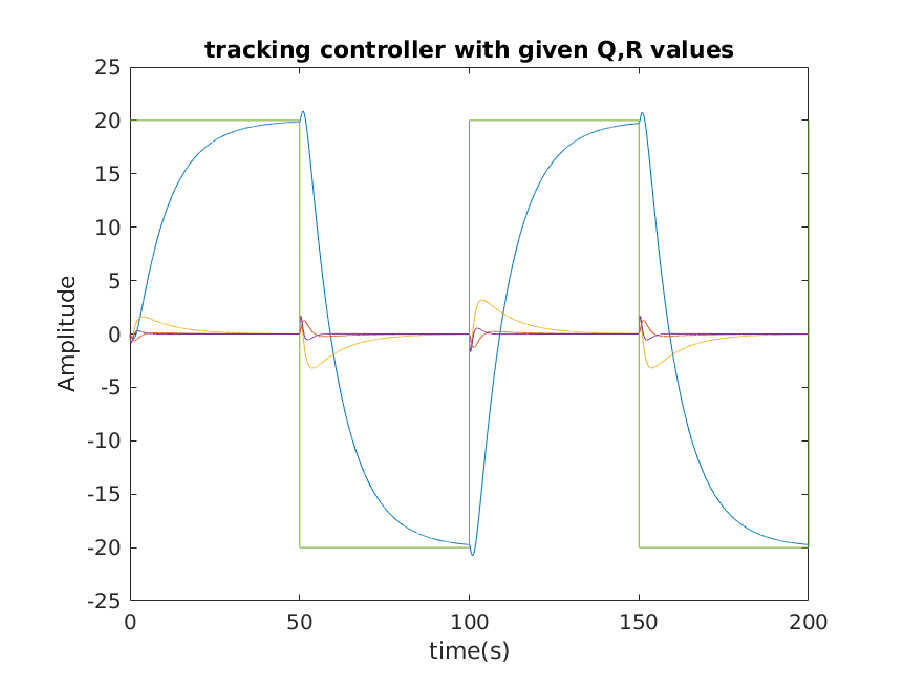
\includegraphics[width=\maxwidth{83.69292523833417em}]{figure_9.eps}
\end{center}


\vspace{1em}
\begin{par}
\begin{flushleft}
\textbf{2 f. Improving the Tracking Controller}
\end{flushleft}
\end{par}

\begin{par}
\begin{flushleft}
The Q and R values can be tuned to track the square wave desired output. It can be improved in the following ways
\end{flushleft}
\end{par}

\begin{enumerate}
\setlength{\itemsep}{-1ex}
   \item{\begin{flushleft} Currently the controlloer is reaching the required amplitude very late. Therefore Q can be increased to reduce convergence time \end{flushleft}}
\end{enumerate}

\begin{matlabcode}
% using t_5 timespan and x_5 initial state specified in 2.d

Q = [[10,0,0,0];[0,5,0,0];[0,0,1,0];[0,0,0,5]];
R = 20;
K = lqr(A, B, Q, R)
\end{matlabcode}
\begin{matlaboutput}
K = 1x4    
   -0.7071   11.2732   -7.7079   10.2244

\end{matlaboutput}
\begin{matlabcode}

v = -1 * inv(C*inv((A-B*K))*B);

[t,x5] = ode45(@(t,x5)(tracking_controller(x5, -K*x5, v, t)), t_5, x_5);
% since y_des is in inches and x5 is in metres, we multiply the x5 plot
plot(t, x5*39.3701)
hold on
plot(t_5,y_des)
hold off
title('improved tracking by changing Q and R')
ylabel('Amplitude')
xlabel('time(s)')
\end{matlabcode}
\begin{center}
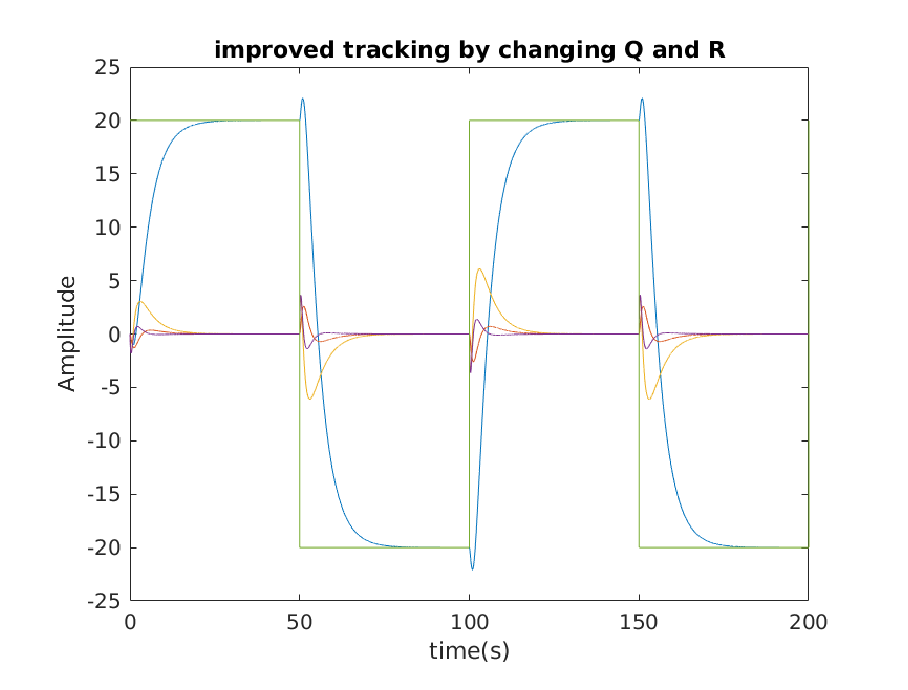
\includegraphics[width=\maxwidth{83.69292523833417em}]{figure_10.eps}
\end{center}


\begin{par}
\begin{flushleft}
Helper functions defined for ode45
\end{flushleft}
\end{par}

\begin{matlabcode}
function x_dot = tracking_controller (x, F, v, t)
xc = x(1);
phi = x(2);
xcdot = x(3);
phidot = x(4);

% constants in the system
gamma = 2;
alpha = 1;
beta = 1;
D = 1;
mu = 3;

% define parameters for y_des
freq=0.01;
offset=0;
amp=20;
duty=50;

% define y_des as a square wave function
y_des = offset+amp*square(2*pi*freq.*t,duty);
u = F + v*y_des;

divisor = ((gamma*alpha) - (beta*beta*cos(phi)*cos(phi)))^(-1);

x_dot = [xcdot;
        phidot;
        divisor*((u*alpha) - (beta*phidot*phidot*sin(phi)*alpha) - (alpha*mu*xcdot) + (beta*D*sin(phi)*cos(phi)));
        divisor*((u*beta*cos(phi)) - (beta*beta*phidot*phidot*sin(phi)*cos(phi)) - (beta*cos(phi)*mu*xcdot) + (gamma*D*sin(phi)))];


% divisor_1 = alpha / ((gamma*alpha) - (beta*beta*cos(phi)*cos(phi)));
% divisor_2 = (beta*cos(phi)) / ((gamma*alpha) - (beta*beta*cos(phi)*cos(phi)));

% x_dot = [xcdot;
%        phidot;
%        divisor_1*(u - (beta*phidot*phidot*sin(phi)) - (mu*xcdot) + ((beta*D*cos(phi)*sin(phi))/alpha));
%        divisor_2*(u - (beta*phidot*phidot*sin(phi)) - (mu*xcdot) + ((gamma*D*sin(phi)) / (beta*cos(phi))))];

end
\end{matlabcode}


\vspace{1em}
\begin{matlabcode}
function x_dot = non_linear_fun (x, u)
xc = x(1);
phi = x(2);
xcdot = x(3);
phidot = x(4);

% constants in the system
gamma = 2;
alpha = 1;
beta = 1;
D = 1;
mu = 3;

divisor = ((gamma*alpha) - (beta*beta*cos(phi)*cos(phi)))^(-1);

x_dot = [xcdot;
        phidot;
        divisor*((u*alpha) - (beta*phidot*phidot*sin(phi)*alpha) - (alpha*mu*xcdot) + (beta*D*sin(phi)*cos(phi)));
        divisor*((u*beta*cos(phi)) - (beta*beta*phidot*phidot*sin(phi)*cos(phi)) - (beta*cos(phi)*mu*xcdot) + (gamma*D*sin(phi)))];


% divisor_1 = alpha / ((gamma*alpha) - (beta*beta*cos(phi)*cos(phi)));
% divisor_2 = (beta*cos(phi)) / ((gamma*alpha) - (beta*beta*cos(phi)*cos(phi)));

% x_dot = [xcdot;
%        phidot;
%        divisor_1*(u - (beta*phidot*phidot*sin(phi)) - (mu*xcdot) + ((beta*D*cos(phi)*sin(phi))/alpha));
%        divisor_2*(u - (beta*phidot*phidot*sin(phi)) - (mu*xcdot) + ((gamma*D*sin(phi)) / (beta*cos(phi))))];

end
\end{matlabcode}

\end{document}
